\documentclass[12pt]{article}

% Generated from frozen study-level 485 cohort (2026-10-14)
\providecommand{\NTech}{485}
\providecommand{\NFull}{375}
\providecommand{\NAbs}{85}
\providecommand{\NMeta}{25}
\providecommand{\NMod}{485}
\providecommand{\NRecent}{375}
\providecommand{\NValTemporal}{81}
\providecommand{\NValRandom}{6}
\providecommand{\NValUnclear}{398}
\providecommand{\NPreTrain}{21}
\providecommand{\NPreFull}{17}
\providecommand{\NPreUnclear}{447}
\providecommand{\NLeakHigh}{32}
\providecommand{\NLeakLow}{7}
\providecommand{\NLeakUnclear}{446}
\providecommand{\NEconomic}{37}
\providecommand{\NStatistical}{48}
\providecommand{\NTransaction}{14}
\providecommand{\NRegimeEval}{8}
\providecommand{\NShockEval}{15}
\providecommand{\NCode}{7}
\providecommand{\NData}{4}

% ============================================================
% PACKAGES
% ============================================================

\usepackage{amsmath,amssymb}
\usepackage{graphicx}
\usepackage{xcolor}
\usepackage{booktabs}
\usepackage{tabularx}
\usepackage{array}
\usepackage{ragged2e}
\usepackage{longtable}
\usepackage{pdflscape}
\usepackage{placeins}
\usepackage{makecell}
\usepackage{caption}
\usepackage{listings}
\usepackage[numbers,sort&compress]{natbib}
\usepackage{tocloft}

% Hyperlinks and named destinations for external cross-references
\usepackage[destlabel=true]{hyperref}

% ============================================================
% COLUMN TYPES AND LONGTABLE ALIGNMENT
% ============================================================

\newcolumntype{L}[1]{%
  >{\RaggedRight\arraybackslash}p{#1}}

\newcolumntype{C}[1]{%
  >{\centering\arraybackslash}p{#1}}

\setlength{\LTleft}{0pt}
\setlength{\LTright}{0pt}

% ============================================================
% SUPPLEMENTARY NUMBERING
% ============================================================

\renewcommand{\thesection}{S\arabic{section}}
\renewcommand{\thesubsection}
  {S\arabic{section}.\arabic{subsection}}
\renewcommand{\thesubsubsection}
  {S\arabic{section}.\arabic{subsection}.\arabic{subsubsection}}

\renewcommand{\thetable}{S\arabic{table}}
\renewcommand{\thefigure}{S\arabic{figure}}

% Equations appear as (S11.1), (S11.2), ...
\numberwithin{equation}{section}
\renewcommand{\theequation}{\thesection.\arabic{equation}}

\setcounter{section}{0}
\setcounter{table}{0}
\setcounter{figure}{0}
\setcounter{equation}{0}

% ============================================================
% TABLE OF CONTENTS SPACING
% ============================================================

\setlength{\cftsecnumwidth}{3.5em}
\setlength{\cftsubsecnumwidth}{5.0em}
\setlength{\cftsubsubsecnumwidth}{6.2em}

% ============================================================
% SEARCH-QUERY LISTING STYLE
% ============================================================

\lstdefinestyle{searchquery}{
    basicstyle=\ttfamily\scriptsize,
    breaklines=true,
    breakatwhitespace=false,
    columns=fullflexible,
    keepspaces=true,
    frame=single,
    numbers=left,
    numberstyle=\tiny,
    numbersep=7pt,
    showstringspaces=false,
    tabsize=2,
    captionpos=t,
    xleftmargin=1.5em,
    framexleftmargin=1.2em,
    aboveskip=1em,
    belowskip=1em
}

% ============================================================
% OPTIONAL TEXT MACROS
% ============================================================

\newcommand{\SuppSecMethodFamilies}
  {Supplementary Section~S11}

\newcommand{\SuppTabFamilyPeriod}
  {Supplementary Table~S20}

\newcommand{\SuppTabFamilyReliability}
  {Supplementary Table~S21}

\providecommand{\bibcommenthead}{}
\begin{document}

\title{
Supplementary Information: Methods, Search Strategies,
Extended Results, Verification, Limitations, and
Method-Family Synthesis\\[3pt]
for\\[3pt]
\textit{Four Decades of Stock Price Prediction:
A Bibliometric, Thematic, and Systematic Review of
Computational Intelligence Approaches}
}

\author{Harmanjeet Singh \and Supreet Singh \and Tarun Kumar \and Amit Kumar  \and S.P.S. Chauhan \and Abhishek S. Verma \and Rohit Salgotra}


\maketitle

\noindent


\tableofcontents
\vspace{1.5em}
\noindent
\paragraph{Supplementary-file organization.}
Sections S1--S11 are presented in this document.
Section S10 contains the extended family-by-family computational synthesis,
while Section S11 reports the extended review limitations and sensitivity
analyses. References cited across all supplementary sections are consolidated
into a single bibliography at the end of this file. The complete mapping among
the 485 frozen coded studies, BibTeX keys, digital object identifiers, principal
method-family assignments, publication periods, and evidence scopes is provided
separately as Supplementary Data S1.

\paragraph{Reference-numbering note.}
Reference numbering in this Supplementary Information is independent of the
numbering used in the main manuscript and follows the order of first citation
across Sections S1--S11.

\clearpage



\section{Evidence bases and denominator map}
\label{sec:supp-denominators}

The analyses reported in the manuscript use several analysis-specific
evidence bases because publication-year validity, keyword availability,
citation and cited-reference coverage, affiliation recoverability, and
technical-synthesis eligibility differ across records. The denominators
defined in Table~\ref{tab:supp-denominators} should not be added
together, and not all evidence bases constitute nested subsets of one
another.

\small
\renewcommand{\arraystretch}{1.15}
\setlength{\tabcolsep}{4pt}

\begin{longtable}{
@{}
L{3.8cm}
C{1.5cm}
L{8.0cm}
@{}
}

\caption{Evidence bases and denominators used across the manuscript
and supplementary analyses.}
\label{tab:supp-denominators}
\\

\toprule
\textbf{Evidence base}
&
\textbf{Records}
&
\textbf{Definition and analytical use}
\\
\midrule
\endfirsthead

\multicolumn{3}{c}{%
\textbf{Table \thetable\ continued from the previous page}}
\\[1mm]

\toprule
\textbf{Evidence base}
&
\textbf{Records}
&
\textbf{Definition and analytical use}
\\
\midrule
\endhead

\midrule
\multicolumn{3}{r}{\textit{Continued on the next page}}
\\
\endfoot

\bottomrule
\endlastfoot

\multicolumn{3}{@{}l}{
\textbf{Panel A. Bibliometric and thematic evidence bases}
}
\\[1mm]

CSV rows entering the cross-database merge
&
8,504
&
Rows assembled before within-source and cross-database duplicate or
overlap removal: \(4{,}832\) from Scopus, \(100\) from Web of
Science, and \(3{,}572\) from five IEEE Xplore query runs.
\\

% Source-specific search and retrieval counts
% &
% Not additive
% &
% Recorded source-level counts were 4,832 for Scopus, 100 for Web of
% Science, 3,572 across five IEEE Xplore query runs, and 826 across six
% ScienceDirect searches. These values should not be summed as unique
% publications because query-run overlap was possible and ScienceDirect
% did not enter the CSV-based merge.
\\

Cross-database deduplicated corpus
&
5,022
&
Unique records retained after DOI-based and normalized-title-based
duplicate or overlap removal. This was the principal evidence base for
descriptive bibliometrics, author collaboration, country collaboration,
source analysis, institutional analysis, and keyword co-occurrence.
\\

Records with a valid publication year
&
5,014
&
Records with a recoverable and analytically valid publication year,
used for annual publication-growth analysis. Eight records without a
valid publication year were excluded only from time-based analyses.
\\

Complete-year corpus, 1987--2025
&
4,610
&
Valid-year records used for thematic mapping and thematic evolution
after excluding 404 records from the incomplete 2026 publication year.
\\

Keyword-bearing complete-year corpus
&
4,528
&
Complete-year records retaining at least one usable normalized author
or index keyword after cleaning and normalization.
\\

Scopus citation-analysis subset
&
4,789
&
Scopus-indexed records containing the citation information used for
document- and source-level citation rankings. Citation values from
different bibliographic databases were not combined.
\\

Reference-preserving Scopus subset
&
4,792
&
Independently deduplicated Scopus records retaining the cited-reference
information required for cited-reference co-citation and document-level
bibliographic-coupling analysis.
\\

Application-area coding set
&
4,974
&
Records containing sufficient title, abstract, keyword, or source
information to support a defensible mutually exclusive primary
application-area classification.
\\

Geocodable affiliation set
&
4,971
&
Application-area records containing at least one affiliation that
could be assigned to a country. Three records without a recoverable
affiliation country were excluded only from geographic analysis.
\\

Priority A1 screening set
&
1,625
&
Records assigned to the strongest rule-based title, abstract, and
keyword relevance category and subjected to detailed screening.
\\

Technical-synthesis suitability set
&
1,553
&
Priority A1 records classified as Include or Maybe and assessed for
technical-synthesis suitability.
\\

\midrule

\multicolumn{3}{@{}l}{
\textbf{Panel B. Technical-synthesis evidence bases}
}
\\[1mm]

Eligible supporting literature not advanced to detailed coding
& 1,059
& Medium-priority ($n=837$) and low-priority ($n=222$) records
retained as supporting literature. \\

High-priority technical-coding candidates
& 494
& Records prioritized for detailed technical coding after
technical-synthesis suitability assessment. \\

Excluded during quality-assessment reconciliation
& 1
& Off-topic title--abstract/metadata mismatch. \\

Initially retained for detailed technical coding
& 493
& High-priority candidates remaining after quality-assessment
reconciliation. \\

Excluded during final full-text reconciliation
& 1
& Non-empirical review article excluded from study-level
methodological analysis. \\

Initial pre-adjudication technical register
& 492
& Canonical study-level register preceding seven further author-approved technical exclusions. \\

Excluded in approved final eligibility adjudication
& 7
& P00332, P00384, P00567, P00681, P00814, P00928, and P01181; excluded only from the technical synthesis. \\

\textbf{Frozen technical-synthesis subset}
& \textbf{485}
& Final author-approved study-level subset used for technical synthesis and methodological audit. \\

\multicolumn{3}{l}{\textbf{Panel C. Evidence-scope and analysis-specific subsets}}\\

Full-text evidence
& 375
& Technical-synthesis studies supported by accessible full-text evidence. \\

Abstract-only evidence
& 85
& Technical-synthesis studies for which coding was limited to the abstract
and available bibliographic information. \\

Metadata-only evidence
& 25
& Technical-synthesis studies for which only bibliographic metadata were
recoverable. \\

Input-modality-applicable subset
& 485
& All retained studies; the previously not-applicable P00814 was excluded from the 485-study technical cohort. \\

\end{longtable}

\normalsize

\noindent
\textit{Notes.}
The review-eligibility window extended through 2026, whereas the
earliest observed publication year in the final corpus was 1987.
Scopus covered 1985--2026, Web of Science covered 1985--2025,
and the IEEE Xplore searches used method-specific starting years
and extended through 2026. The complete-year thematic corpus
therefore covers 1987--2025 and excludes the incomplete 2026
publication year.

The evidence bases are analysis specific. Some are nested, including
the valid-year, complete-year, and keyword-bearing complete-year
corpora. Others, including the citation-analysis, reference-preserving,
application-area, and geocodable-affiliation sets, were constructed
independently according to the metadata needed for each analysis.

\FloatBarrier
\clearpage

% \paragraph{Interpretive boundary of method-family coverage.}
% The database expressions were complementary rather than syntactically
% equivalent. Scopus supplied the principal bibliometric stream, while
% the IEEE Xplore runs explicitly extended retrieval to recurrent,
% convolutional, transformer, attention, sentiment/NLP, and
% metaheuristic terminology. The final study-level register confirms
% representation of these method families, but it does not permit a
% database-specific recall calculation because individual-study
% retrieval provenance was not retained consistently in the final
% technical register. Accordingly, no claim of exhaustive
% method-family retrieval is made.

\section{Database-specific search strategies}
\label{sec:supp-search}

This section reports the executable database queries, field-code
adaptations, search periods, recorded counts, and source-specific
provenance information used during evidence identification.

The overall review-eligibility window was 1985--2026, while search
execution was database specific. Scopus covered 1985--2026,
Web of Science covered 1985--2025, and the five IEEE Xplore query
runs used method-specific starting years and extended through 2026.

Scopus, Web of Science, and IEEE Xplore contributed rows to the
initial identification set. The query expressions are reproduced
from the recovered contemporaneous search audit. Where an interface
required multiple queries, each recorded expression is reported
separately rather than being reconstructed as a single retrospective
query.
\subsection{Scopus search expression}
\label{sec:supp-scopus-query}

Scopus was searched through the \texttt{TITLE-ABS-KEY} field using a
forecasting-task block and a computational-intelligence block. The
recorded search period was 1985--2026, and 4,832 records contributed
to the CSV-based merge.

\begin{lstlisting}[
style=searchquery,
caption={Executable Scopus search expression recorded in the search
audit.},
label={lst:supp-scopus-query}
]
TITLE-ABS-KEY(
(
    "stock price prediction" OR
    "stock price forecasting" OR
    "stock market prediction" OR
    "stock market forecasting" OR
    "share price prediction" OR
    "share price forecasting" OR
    "equity price prediction" OR
    "equity price forecasting"
)
AND
(
    "computational intelligence" OR
    "artificial intelligence" OR
    "machine learning" OR
    "deep learning" OR
    "neural network" OR
    "neural networks" OR
    "artificial neural network" OR
    "support vector machine" OR
    "support vector regression" OR
    "random forest" OR
    "decision tree" OR
    "gradient boosting" OR
    "XGBoost" OR
    "LightGBM"
)
)
\end{lstlisting}

\subsection{Web of Science search expression}
\label{sec:supp-wos-query}

Web of Science was searched through the Topic field. The recorded
settings were English language; articles, proceedings papers, books,
and book chapters; and publication years 1985--2025. The search was
executed on 19 June 2026, and the archived export contained 100
records.

\begin{lstlisting}[
style=searchquery,
caption={Web of Science Topic-field expression recorded in the search
audit.},
label={lst:supp-wos-query}
]
TS=(
  "stock price prediction" OR
  "stock price forecasting" OR
  "stock market prediction" OR
  "stock market forecasting" OR
  "financial time series forecasting" OR
  "equity price prediction" OR
  "share price prediction"
)
AND
TS=(
  "machine learning" OR
  "deep learning" OR
  "computational intelligence" OR
  "artificial intelligence" OR
  "neural network" OR
  "LSTM" OR
  "GRU" OR
  "CNN" OR
  "transformer" OR
  "attention mechanism" OR
  "graph neural network" OR
  "sentiment analysis" OR
  "multimodal" OR
  "metaheuristic" OR
  "evolutionary optimization" OR
  "feature selection" OR
  "hyperparameter optimization"
)
\end{lstlisting}

The recorded Web of Science expression used separate Topic-field blocks
for the forecasting task and computational-method terminology, linked by
the Boolean operator AND. The Web of Science strategy included additional
forecasting and computational-method terms relative to the recorded Scopus
expression. All exported records were subsequently subjected to the common
title--abstract eligibility-screening and duplicate-resolution procedures.

\subsection{IEEE Xplore search expression}
\label{sec:supp-ieee-query}


IEEE Xplore was searched through five complementary query runs covering
broad machine-learning and deep-learning methods, recurrent and
convolutional architectures, transformer and attention mechanisms,
sentiment and textual information, and metaheuristic optimization.
Conference and journal publications were retained.

The five query-run outputs were assembled into the initial CSV workflow.
Because the expressions were complementary but potentially overlapping,
the \(3{,}572\) rows were subjected to the same subsequent duplicate
and overlap-removal procedure as the other database records.
Supplementary Table~\ref{tab:supp-ieee-query-summary} reports the exact
query expressions and raw result counts.

\begin{landscape}
\begin{table}[!p]
\centering
\caption{IEEE Xplore query runs used to retrieve computational
stock-market forecasting studies.}
\label{tab:supp-ieee-query-summary}

\footnotesize
\setlength{\tabcolsep}{4pt}
\renewcommand{\arraystretch}{1.18}

\begin{tabularx}{\linewidth}{
@{}
>{\centering\arraybackslash}p{1.2cm}
>{\RaggedRight\arraybackslash}X
>{\centering\arraybackslash}p{2.1cm}
>{\centering\arraybackslash}p{2.7cm}
>{\centering\arraybackslash}p{1.7cm}
@{}
}
\toprule
\textbf{Run}
&
\textbf{Executed search expression}
&
\textbf{Year range}
&
\textbf{Publication types}
&
\textbf{Raw results}
\\
\midrule

Q1
&
\texttt{("stock price prediction" OR "stock market prediction" OR
"stock price forecasting") AND ("machine learning" OR
"deep learning")}
&
1991--2026
&
Conferences and journals
&
1,547
\\

Q2
&
\texttt{("stock price prediction" OR "stock market prediction") AND
(LSTM OR GRU OR CNN OR "convolutional neural network")}
&
2005--2026
&
Conferences and journals
&
1,161
\\

Q3
&
\texttt{("stock price prediction" OR "stock market forecasting") AND
(transformer OR "attention mechanism" OR "self-attention")}
&
2004--2026
&
Conferences and journals
&
189
\\

Q4
&
\texttt{("stock price prediction" OR "stock market prediction") AND
("sentiment analysis" OR "financial news" OR NLP OR
"natural language processing")}
&
2008--2026
&
Conferences and journals
&
602
\\

Q5
&
\texttt{("stock price prediction" OR "stock market forecasting") AND
(metaheuristic OR "genetic algorithm" OR
"particle swarm optimization" OR "grey wolf optimizer")}
&
2004--2026
&
Conferences and journals
&
73
\\

\midrule
\multicolumn{4}{r}{\textbf{Total query-run rows}}
&
\textbf{3,572}
\\

\bottomrule
\end{tabularx}

\vspace{1.5mm}

\begin{minipage}{\linewidth}
\footnotesize
\textit{Note.}
The five queries were complementary but potentially overlapping. The
recorded counts sum to \(3{,}572\) query-run rows:

\[
1{,}547+1{,}161+189+602+73=3{,}572.
\]

Accordingly, this total represents rows assembled from the five query
runs before the subsequent within- and cross-database duplicate or
overlap removal stage. It should not be interpreted as a confirmed
count of \(3{,}572\) unique IEEE Xplore publications. The year ranges
are reproduced from the contemporaneous search audit.
\end{minipage}


\end{table}
\end{landscape}
\FloatBarrier

% \subsubsection{IEEE Xplore Query 1: broad machine and deep learning}

% \begin{lstlisting}[
% style=searchquery,
% caption={IEEE Xplore Query 1.},
% label={lst:supp-ieee-query-1}
% ]
% ("stock price prediction" OR
%  "stock market prediction" OR
%  "stock price forecasting")
% AND
% ("machine learning" OR "deep learning")
% \end{lstlisting}

% The query returned 1,547 conference and journal records within the
% recorded 1991--2026 range.

% \subsubsection{IEEE Xplore Query 2: recurrent and convolutional models}

% \begin{lstlisting}[
% style=searchquery,
% caption={IEEE Xplore Query 2.},
% label={lst:supp-ieee-query-2}
% ]
% ("stock price prediction" OR
%  "stock market prediction")
% AND
% (LSTM OR GRU OR CNN OR
%  "convolutional neural network")
% \end{lstlisting}

% The query returned 1,161 conference and journal records within the
% reported 2005--2026 range.

% \subsubsection{IEEE Xplore Query 3: transformer and attention models}

% \begin{lstlisting}[
% style=searchquery,
% caption={IEEE Xplore Query 3.},
% label={lst:supp-ieee-query-3}
% ]
% ("stock price prediction" OR
%  "stock market forecasting")
% AND
% (transformer OR
%  "attention mechanism" OR
%  "self-attention")
% \end{lstlisting}

% The query returned 189 conference and journal records within the
% reported 2004--2026 range.

% \subsubsection{IEEE Xplore Query 4: sentiment and textual information}

% \begin{lstlisting}[
% style=searchquery,
% caption={IEEE Xplore Query 4.},
% label={lst:supp-ieee-query-4}
% ]
% ("stock price prediction" OR
%  "stock market prediction")
% AND
% ("sentiment analysis" OR
%  "financial news" OR
%  NLP OR
%  "natural language processing")
% \end{lstlisting}

% The query returned 602 conference and journal records within the
% reported 2008--2026 range.

% \subsubsection{IEEE Xplore Query 5: metaheuristic optimization}

% \begin{lstlisting}[
% style=searchquery,
% caption={IEEE Xplore Query 5.},
% label={lst:supp-ieee-query-5}
% ]
% ("stock price prediction" OR
%  "stock market forecasting")
% AND
% (metaheuristic OR
%  "genetic algorithm" OR
%  "particle swarm optimization" OR
%  "grey wolf optimizer")
% \end{lstlisting}

% The query returned 73 conference and journal records within the
% reported 2004--2026 range.

The five IEEE Xplore query runs, including the complete search
expressions, publication-year ranges, publication types, and recorded
query-run counts, are reported in Table~S2. Because the runs were
complementary but potentially overlapping, their summed count represents
query-run rows prior to duplicate and overlap removal rather than a count
of unique IEEE Xplore publications.

\subsubsection{Interpretation of the IEEE Xplore query-run total}

The five recorded IEEE Xplore query-run counts summed to
\(3{,}572\):

\[
1{,}547+1{,}161+189+602+73=3{,}572.
\]

The query expressions were complementary and potentially overlapping.
Accordingly, the value \(3{,}572\) is treated as the number of
query-run rows assembled before the subsequent within- and
cross-database duplicate or overlap removal stage, rather than as a
confirmed count of \(3{,}572\) unique publications.

\clearpage

% \subsection{ScienceDirect search expressions}
% \label{sec:supp-sciencedirect-query}

% ScienceDirect retrieval used six complementary search expressions
% covering broad machine- and deep-learning methods, neural-network
% models, recurrent and convolutional architectures, transformer and
% attention mechanisms, textual and sentiment information, and
% metaheuristic optimization. The recorded search period was
% 1985--2025, and the contemporaneous search log reported 826 records.

% Because the six search expressions were conceptually overlapping, the
% value 826 is reported as the archived ScienceDirect retrieval count
% rather than as a confirmed count of 826 unique publications.
% ScienceDirect records were exported through RIS or BibTeX, imported
% into Zotero, and used for reference enrichment, duplicate verification,
% and full-text evidence recovery. They were not included in the
% \(8{,}504\)-row CSV-based bibliometric merge.

% \subsubsection{ScienceDirect Query 1: broad machine and deep learning}

% \begin{lstlisting}[
% style=searchquery,
% caption={ScienceDirect Query 1: machine- and deep-learning search.},
% label={lst:supp-sd-query-1}
% ]
% "stock price prediction"
% AND
% ("machine learning" OR "deep learning")
% \end{lstlisting}

% \subsubsection{ScienceDirect Query 2: stock-market forecasting and
% neural-learning methods}

% \begin{lstlisting}[
% style=searchquery,
% caption={ScienceDirect Query 2: stock-market forecasting and
% neural-learning methods.},
% label={lst:supp-sd-query-2}
% ]
% "stock market forecasting"
% AND
% ("machine learning" OR
%  "deep learning" OR
%  "neural network")
% \end{lstlisting}

% \subsubsection{ScienceDirect Query 3: recurrent and convolutional
% architectures}

% \begin{lstlisting}[
% style=searchquery,
% caption={ScienceDirect Query 3: recurrent and convolutional models.},
% label={lst:supp-sd-query-3}
% ]
% "stock price prediction"
% AND
% (LSTM OR GRU OR CNN)
% \end{lstlisting}

% \subsubsection{ScienceDirect Query 4: transformer and attention
% mechanisms}

% \begin{lstlisting}[
% style=searchquery,
% caption={ScienceDirect Query 4: transformer and attention models.},
% label={lst:supp-sd-query-4}
% ]
% "stock price prediction"
% AND
% (transformer OR "attention mechanism")
% \end{lstlisting}

% \FloatBarrier


% \subsubsection{ScienceDirect Query 5: sentiment and textual
% information}

% \begin{lstlisting}[
% style=searchquery,
% caption={ScienceDirect Query 5: sentiment and textual information.},
% label={lst:supp-sd-query-5}
% ]
% "stock price prediction"
% AND
% ("sentiment analysis" OR
%  "financial news" OR
%  NLP)
% \end{lstlisting}
% \FloatBarrier




% \subsubsection{ScienceDirect Query 6: metaheuristic optimization}

% \begin{lstlisting}[
% style=searchquery,
% caption={ScienceDirect Query 6: metaheuristic optimization.},
% label={lst:supp-sd-query-6}
% ]
% "stock price prediction"
% AND
% (metaheuristic OR
%  "genetic algorithm" OR
%  "particle swarm optimization" OR
%  "grey wolf optimizer")
% \end{lstlisting}
% \FloatBarrier

% \begin{table}[!htbp]
% \centering
% \caption{ScienceDirect search execution and analytical use.}
% \label{tab:supp-sciencedirect-summary}

% \small
% \setlength{\tabcolsep}{5pt}
% \renewcommand{\arraystretch}{1.15}

% \begin{tabularx}{\linewidth}{
% @{}
% >{\RaggedRight\arraybackslash}p{3.4cm}
% >{\RaggedRight\arraybackslash}X
% @{}
% }
% \toprule
% \textbf{Search characteristic}
% &
% \textbf{Recorded information}
% \\
% \midrule

% Search structure
% &
% Six complementary queries covering machine learning, deep learning,
% neural networks, recurrent and convolutional models, transformers,
% attention mechanisms, sentiment and textual information, and
% metaheuristic optimization.
% \\

% Recorded publication period
% &
% 1985--2025.
% \\

% Archived retrieval count
% &
% 826 records across the documented ScienceDirect searches.
% \\

% Export formats
% &
% RIS and BibTeX.
% \\

% Reference-management workflow
% &
% Imported into Zotero for reference enrichment, duplicate verification,
% and full-text evidence organization.
% \\

% Contribution to the \(8{,}504\)-row CSV merge
% &
% None. ScienceDirect records were handled separately and were not
% included in the CSV-based bibliometric merge.
% \\

% Analytical use
% &
% Reference enrichment, duplicate verification, bibliography management,
% and full-text evidence recovery for systematic technical synthesis.
% \\

% \bottomrule
% \end{tabularx}

% \vspace{1mm}

% \begin{minipage}{\linewidth}
% \footnotesize
% \textit{Note.}
% The six ScienceDirect expressions were potentially overlapping.
% Accordingly, the recorded count of 826 should not be interpreted as a
% verified count of unique ScienceDirect publications unless a separate
% within-ScienceDirect deduplication audit confirms uniqueness.
% \end{minipage}

% \end{table}
\FloatBarrier
\section{Supplementary Descriptive Bibliometric Results}
\label{sec:supp-descriptive-bibliometric-results}
\FloatBarrier

\begin{figure}[htbp]
    \centering
    \includegraphics[width=0.90\textwidth]{Fig_Document_Type_Distribution_Final.pdf}
    \caption{Document-type distribution of the stock price prediction literature based on the deduplicated bibliometric corpus. Counts and percentages are calculated from the merged Scopus, Web of Science, and IEEE Xplore records after duplicate removal.}
    \label{fig:document-type-distribution}
\end{figure}

\begin{table}[htbp]
\centering
\caption{Top 10 productive authors in stock price prediction research}
\label{tab:top-productive-authors}
\begin{tabular}{p{0.7cm}p{2.6cm}r r r}
\toprule
\textbf{Rank} & \textbf{Author} & \textbf{Publications} & \textbf{Total citations} & \textbf{Avg. citations} \\
\midrule
1 & Wang Y. & 50 & 1195 & 23.90 \\
2 & Chen Y. & 43 & 1020 & 23.72 \\
3 & Li Y. & 42 & 1240 & 29.52 \\
4 & Wang J. & 33 & 2454 & 74.36 \\
5 & Zhang Y. & 33 & 1722 & 52.18 \\
6 & Liu Y. & 29 & 920 & 31.72 \\
7 & Singh S. & 28 & 459 & 16.39 \\
8 & Li X. & 27 & 1313 & 48.63 \\
9 & Wang L. & 26 & 263 & 10.12 \\
10 & Li J. & 25 & 1595 & 63.80 \\
\bottomrule
\end{tabular}
\end{table}
\FloatBarrier



\begin{table*}[htbp]
\centering
\caption{Top 10 contributing institutions in stock price prediction research}
\label{tab:top-institutions}
\begin{tabular}{p{0.8cm}p{6.2cm}r r r}
\toprule
\textbf{Rank} & \textbf{Institution} & \textbf{Publications} & \textbf{Total citations} & \textbf{Avg. citations} \\
\midrule
1 & Bina Nusantara University & 58 & 401 & 6.91 \\
2 & Vellore Institute of Technology & 52 & 769 & 14.79 \\
3 & Chandigarh University & 37 & 63 & 1.70 \\
4 & National Institute of Technology & 35 & 1205 & 34.43 \\
5 & SRM Institute of Science and Technology & 28 & 126 & 4.50 \\
6 & Lovely Professional University & 27 & 66 & 2.44 \\
7 & Nanyang Technological University & 25 & 1073 & 42.92 \\
8 & Central University of Finance and Economics & 25 & 299 & 11.96 \\
9 & Amity University & 25 & 202 & 8.08 \\
10 & Amrita Vishwa Vidyapeetham & 25 & 154 & 6.16 \\
\bottomrule
\end{tabular}
\end{table*}
\FloatBarrier

\section{Supplementary Collaboration Networks}
\label{sec:supp-collaboration-networks}
\begin{figure}[!htbp]
    \centering
    \includegraphics[
        width=\textwidth,
        trim=10 10 10 10,
        clip
    ]{Fig_Author_Coauthorship_Network_Final.pdf}
    \caption{Author-level co-authorship network in stock price prediction research. The network contains 275 retained bibliographic author-name entities distributed across 19 collaboration clusters, with 1164 co-authorship links and a total link strength of 866.00. All retained entities belong to a single connected component, with no isolated nodes. Node size represents publication output, link thickness denotes fractional co-authorship strength, and colours identify collaboration clusters generated by VOSviewer. The network is globally connected but highly modular, containing several visually distinct collaboration communities linked through comparatively sparse bridging relationships.}
    \label{fig:author-coauthorship-network}
\end{figure}
\FloatBarrier

\begin{figure}[!htbp]
    \centering
    \includegraphics[
        width=\textwidth,
        trim=10 10 10 10,
        clip
    ]{Fig_Country_Collaboration_Overlay_Final.pdf}
    \caption{Temporal overlay visualization of the country-level collaboration network in stock price prediction research. Node size represents country-level publication output, link thickness denotes fractional collaboration strength, and node colour indicates the average publication year of the documents associated with each country. The overall review-eligibility window was 1985--2026, while the
retained bibliometric corpus spans 1987--2026. Database-specific
search-execution periods are reported in Supplementary Information, Section~S2.}
    \label{fig:country-collaboration-overlay}
\end{figure}
\FloatBarrier


\FloatBarrier
\section{Supplementary Science-Mapping Settings}
\label{sec:supp-science-mapping-settings}



\begin{table}[htbp]
\centering
\caption{VOSviewer settings for author-level co-authorship analysis}
\label{tab:author-coauthorship-settings}
\begin{tabular}{p{6.2cm}p{6.0cm}}
\toprule
\textbf{Parameter} & \textbf{Setting} \\
\midrule
Analysis type & Author-level co-authorship analysis \\
Unit of analysis & Bibliographic author-name entities \\
Counting method & Fractional counting \\
Minimum documents per author-name entity & 5 \\
Minimum citations per author-name entity & 49 \\
Maximum authors per document & 25 \\
Bibliometric corpus & 5022 deduplicated records \\
Retained author-name entities & 275 \\
Connected components & 1 \\
Largest connected component & 275 author-name entities \\
Isolated author-name entities & 0 \\
Collaboration clusters & 19 \\
Co-authorship links & 1164 \\
Total link strength & 866.00 \\
Visualization software & VOSviewer version 1.6.21 \\
\bottomrule
\end{tabular}
\end{table}
\FloatBarrier

\begin{table}[htbp]
\centering
\caption{VOSviewer settings for the country collaboration analysis}
\label{tab:country-collaboration-settings}
\begin{tabular}{p{6.0cm}p{6.2cm}}
\toprule
\textbf{Parameter} & \textbf{Setting} \\
\midrule
Analysis type & Country-level co-authorship analysis \\
Unit of analysis & Countries \\
Network weighting & Fractional collaboration links \\
Node weight & Number of documents \\
Minimum documents per country & 10 \\
Bibliometric corpus & 5022 deduplicated records \\
Countries retained & 48 \\
Collaboration clusters & 6 \\
Collaboration links & 322 \\
Total link strength & 731.00 \\
Overlay score & Average publication year \\
Displayed overlay range & 2019--2023 \\
Review-eligibility window
&1985--2026\\
Database-specific search execution&
Scopus: 1985--2026; Web of Science: 1985--2025;
IEEE Xplore: run-specific starting years through 2026
\\
Observed publication period & 1987--2026 \\
Visualization software & VOSviewer version 1.6.21 \\
\bottomrule
\end{tabular}
\end{table}
\FloatBarrier


\FloatBarrier
\section{Supplementary Thematic-Evolution Details}
\label{sec:supp-thematic-evolution-details}

\begin{table}[!htbp]
\centering
\caption{Publication periods used for thematic-evolution analysis.}
\label{tab:thematic_evolution_periods}
\begin{tabular}{lrr}
\toprule
\textbf{Period} &
\textbf{Documents} &
\textbf{Share (\%)} \\
\midrule
1987--2005 & 107 & 2.32 \\
2006--2015 & 404 & 8.76 \\
2016--2020 & 752 & 16.31 \\
2021--2022 & 861 & 18.68 \\
2023--2024 & 1,391 & 30.17 \\
2025 & 1,095 & 23.75 \\
\bottomrule
\textbf{Total} & \textbf{4,610} & \textbf{100.00} \\
\hline
\end{tabular}
\end{table}
\FloatBarrier


\FloatBarrier
\section{Supplementary Technical-Synthesis Tables}
\label{sec:supp-technical-synthesis-tables}
\begin{table}[!htbp]
\centering
\caption{Distribution of primary forecasting targets in the frozen $n=485$ technical-synthesis subset.}
\label{tab:supp-target-distribution}
\small
\setlength{\tabcolsep}{4pt}
\renewcommand{\arraystretch}{1.12}
\begin{tabular}{lrr}
\toprule
Forecasting target & Studies & Share (\%) \\
\midrule
Price level & 378 & 77.9 \\
Return & 17 & 3.5 \\
Direction & 47 & 9.7 \\
Volatility & 1 & 0.2 \\
Trend or regime & 8 & 1.6 \\
Multi-target & 32 & 6.6 \\
Not reported & 2 & 0.4 \\
\textbf{Total} & \textbf{485} & \textbf{100.0} \\
\bottomrule
\end{tabular}

\vspace{1mm}
\begin{minipage}{0.97\linewidth}
\footnotesize
\textit{Note.} Percentages use all 485 retained studies. Not reported denotes insufficient evidence to assign a financial prediction target.
\end{minipage}
\end{table}

\FloatBarrier

\begin{table}[!htbp]
\centering
\caption{Distribution of forecast horizons in the frozen $n=485$ technical synthesis.}
\label{tab:supp-horizon-distribution}
\small
\setlength{\tabcolsep}{4pt}
\renewcommand{\arraystretch}{1.12}
\begin{tabular}{lrrr}
\toprule
Forecast horizon & Studies & Share of all (\%) & Share reported (\%) \\
\midrule
Intraday & 17 & 3.5 & 10.1 \\
One trading day & 79 & 16.3 & 47.0 \\
Short multi-day: 2--5 days & 4 & 0.8 & 2.4 \\
Weekly: 6--10 trading days & 11 & 2.3 & 6.5 \\
Monthly: 11--22 trading days & 4 & 0.8 & 2.4 \\
Longer than one month & 9 & 1.9 & 5.4 \\
Multiple forecast horizons & 44 & 9.1 & 26.2 \\
\textbf{Reported subtotal} & \textbf{168} & \textbf{34.6} & \textbf{100.0} \\
Not reported & 317 & 65.4 & -- \\
\textbf{Total} & \textbf{485} & \textbf{100.0} & -- \\
\bottomrule
\end{tabular}

\vspace{1mm}
\begin{minipage}{0.97\linewidth}
\footnotesize
\textit{Note.} Within-reported percentages use 168 identifiable forecast horizons; input window length and sampling frequency do not define the forecast lead.
\end{minipage}
\end{table}

\FloatBarrier

\begin{table}[!htbp]
\centering
\caption{Distribution of asset scope in the frozen $n=485$ technical synthesis.}
\label{tab:supp-asset-scope}
\small
\setlength{\tabcolsep}{4pt}
\renewcommand{\arraystretch}{1.12}
\begin{tabular}{lrrr}
\toprule
Asset scope & Studies & Share of all (\%) & Share identified (\%) \\
\midrule
Single stock & 103 & 21.2 & 29.4 \\
Multiple stocks & 153 & 31.5 & 43.7 \\
Single stock index & 62 & 12.8 & 17.7 \\
Multiple indices & 19 & 3.9 & 5.4 \\
Portfolio & 1 & 0.2 & 0.3 \\
Cross-market & 12 & 2.5 & 3.4 \\
\textbf{Identifiable subtotal} & 350 & 72.2 & 100.0 \\
Not reported & 135 & 27.8 & -- \\
\textbf{Total} & \textbf{485} & \textbf{100.0} & -- \\
\bottomrule
\end{tabular}

\vspace{1mm}
\begin{minipage}{0.97\linewidth}
\footnotesize
\textit{Note.} All-study percentages use n=485; within-identified percentages use n=350. No asset scope is inferred solely from a data-provider name.
\end{minipage}
\end{table}


\begin{table}[!htbp]
\centering
\caption{Study-level leakage-signal categories in the frozen $n=485$ technical-synthesis subset.}
\label{tab:supp-leakage-mechanisms}
\small
\setlength{\tabcolsep}{4pt}
\renewcommand{\arraystretch}{1.12}
\begin{tabular}{lrr}
\toprule
Leakage-signal status & Studies & Share (\%) \\
\midrule
At least one passage-verified signal & 32 & 6.6 \\
No explicit passage-verified signal identified & 7 & 1.4 \\
Specific leakage mechanism not classifiable & 446 & 92.0 \\
\textbf{Total} & \textbf{485} & \textbf{100.0} \\
\bottomrule
\end{tabular}

\vspace{1mm}
\begin{minipage}{0.97\linewidth}
\footnotesize
\textit{Note.} Mechanism-specific non-mutually-exclusive counts from the earlier 492-study corpus are not reproduced because the frozen 51-field register does not store the per-study mechanism assignments. The present table reports only independently reproducible study-level statuses.
\end{minipage}
\end{table}

\FloatBarrier   



\begin{table}[!htbp]
\centering
\caption{Reconciled leakage-signal status by overall study-level leakage risk in the frozen $n=485$ technical subset.}
\label{tab:supp-leakage-signal-risk-crosswalk}
\small
\setlength{\tabcolsep}{4pt}
\renewcommand{\arraystretch}{1.12}
\begin{tabular}{lrrrr}
\toprule
Leakage-signal status & High & Low & Unclear & Total \\
\midrule
At least one passage-verified signal & 32 & 0 & 0 & 32 \\
No explicit passage-verified signal & 0 & 7 & 0 & 7 \\
Specific mechanism not classifiable & 0 & 0 & 446 & 446 \\
Total & 32 & 7 & 446 & 485 \\
\bottomrule
\end{tabular}

\vspace{1mm}
\begin{minipage}{0.97\linewidth}
\footnotesize
\textit{Note.} The signal and risk variables are distinct; the equality of totals results from the audited frozen coding.
\end{minipage}
\end{table}


Within the representative recent reviews examined in
Supplementary Table~S13, we did not identify another review that combined
cross-database bibliometric performance analysis, multiple science-mapping
perspectives, thematic evolution, and a study-level audit of validation,
preprocessing boundaries, leakage, economic evaluation, and reproducibility
within a single review design.

\section{Extended review protocol and coding verification}
\label{sec:supp-review-protocol-and-coding-verification}

% Existing supplementary tables are S1--S12.
% Therefore, the next table must be Table S13.
\setcounter{table}{12}

This section provides the extended comparison with recent reviews,
the complete technical-extraction and methodological-audit fields,
and the detailed coding-verification and adjudication procedure.
These materials support the concise methodological description
retained in the main manuscript.

\paragraph{Final input-modality applicability.}
The historical 492-study register included P00814 as modality-not-applicable.
This record was subsequently among the seven author-approved technical
exclusions. Accordingly all 485 retained studies are applicable to the
final input-modality prevalence analysis; 451 have at least one
recoverable modality and 34 remain unclassified for lack of evidence.
The modality denominator is now identical to the 485-study technical
denominator, while all non-technical bibliometric denominators are unchanged.

\subsection{Comparison with representative recent reviews}
\label{sec:supp-review-comparison}

Representative recent reviews differ in publication period, corpus size,
methodological coverage, science-mapping scope, and the extent to which
they assess validation, data leakage, economic evaluation, and
reproducibility. Table~\ref{tab:supp-review-comparison} compares the
present review with five representative recent reviews selected to reflect
bibliometric, systematic, neural-network, evolutionary-optimization, and
broad computational-forecasting perspectives.

The comparison is intended to establish the methodological positioning of
the present review rather than to rank the scientific quality of previous
reviews. A review was coded as addressing a comparison dimension only when
that dimension was treated as an explicit analytical component rather than
being mentioned incidentally.


\begin{landscape}

\small
\setlength{\tabcolsep}{3pt}
\renewcommand{\arraystretch}{1.15}

\begin{longtable}{
@{}
>{\RaggedRight\arraybackslash}p{3.0cm}
>{\RaggedRight\arraybackslash}p{3.5cm}
>{\RaggedRight\arraybackslash}p{8.2cm}
>{\centering\arraybackslash}p{1.15cm}
>{\centering\arraybackslash}p{1.15cm}
>{\centering\arraybackslash}p{1.15cm}
>{\centering\arraybackslash}p{1.15cm}
>{\centering\arraybackslash}p{1.15cm}
@{}
}

\caption{Comparison of the present review with representative recent
reviews of computational stock-market forecasting.}
\label{tab:supp-review-comparison}
\\

\toprule
\textbf{Review}
&
\textbf{Review period and corpus}
&
\textbf{Primary scope}
&
\textbf{BA}
&
\textbf{SM}
&
\textbf{TS}
&
\textbf{VLA}
&
\textbf{RA}
\\
\midrule
\endfirsthead

\multicolumn{8}{c}{
\textbf{Table~\thetable\ continued from the previous page}
}
\\[1mm]

\toprule
\textbf{Review}
&
\textbf{Review period and corpus}
&
\textbf{Primary scope}
&
\textbf{BA}
&
\textbf{SM}
&
\textbf{TS}
&
\textbf{VLA}
&
\textbf{RA}
\\
\midrule
\endhead

\midrule
\multicolumn{8}{r}{\textit{Continued on the next page}}
\\
\endfoot

\bottomrule
\endlastfoot


Vuong et al. (2024)
\cite{Vuong2024Bibliometric}
&
Period not explicitly bounded; \(n=73\)
&
ARIMA, conventional machine learning, deep learning, and hybrid
forecasting based mainly on historical prices and technical indicators.
&
Partial
&
No
&
Yes
&
No
&
No
\\[2mm]


Thakkar and Chaudhari (2024)
\cite{thakkar2024genetic}
&
2013--2022; final \(n\) not explicitly reported
&
Genetic algorithms for parameter optimization, feature selection,
stock-price and trend prediction, portfolio optimization, and hybrid
evolutionary models.
&
No
&
No
&
Yes
&
No
&
No
\\[2mm]


Bao et al. (2025)
\cite{bao2025datadriven}
&
2015--2023; \(n=63\)
&
Neural forecasting using RNNs, CNNs, transformers, GNNs, GANs, and
LLMs, together with commonly used datasets and evaluation measures.
&
No
&
No
&
Yes
&
No
&
No
\\[2mm]


Shafiei Hafshejani and Mansouri (2026)
\cite{hafshejani2026lstm}
&
2018--2024; \(n=98\)
&
LSTM forecasting, preprocessing, input features, architecture design,
market coverage, parameter settings, performance measures, and hybrid
LSTM models.
&
No
&
No
&
Yes
&
No
&
No
\\[2mm]


Darwish et al. (2026)
\cite{darwish2026stock}
&
Recent literature; publication period and final \(n\) not explicitly
reported
&
Feature engineering, machine learning, deep learning, ensemble and
hybrid approaches, textual forecasting, reinforcement learning,
multi-agent reinforcement learning, large language models,
explainability, and financial agents.
&
No
&
No
&
Yes
&
No
&
No
\\[2mm]


\textbf{Present review}
&
\textbf{1987--2026 bibliometric corpus, \(n=5{,}022\);
2016--2026 technical subset, \(n=485\)}
&
\textbf{Integrated bibliometric, thematic, and systematic review of
statistical models, machine learning, deep learning, hybrid architectures,
transformers, graph models, sentiment and multimodal systems,
metaheuristics, explainability, uncertainty quantification, validation
design, data leakage, economic evaluation, and reproducibility.}
&
\textbf{Yes}
&
\textbf{Yes}
&
\textbf{Yes}
&
\textbf{Yes}
&
\textbf{Yes}
\\

\end{longtable}


\begin{minipage}{0.98\linewidth}
\footnotesize
\textit{Notes.}
BA = bibliometric analysis;
SM = science mapping or thematic evolution;
TS = technical synthesis;
VLA = study-level validation and leakage audit;
RA = reproducibility audit.

``Partial'' denotes descriptive bibliometric analysis without
network-based science mapping. SM requires analyses such as
co-authorship, co-citation, bibliographic coupling, keyword
co-occurrence, thematic mapping, or thematic evolution. VLA requires
systematic study-level assessment of temporal splitting, preprocessing
boundaries, target construction, or information leakage. RA requires
systematic assessment of code, data, configurations, software
environments, random seeds, or implementation availability.

Formal journal-volume years are reported. Shafiei Hafshejani and
Mansouri and Darwish et al. were published online in 2025 but assigned
to 2026 journal volumes.

The comparison identifies analytical coverage within the selected
representative reviews and should not be interpreted as a ranking of
their overall scientific quality.
\end{minipage}

\end{landscape}

\FloatBarrier


% ------------------------------------------------------------
% S8.2 TECHNICAL EXTRACTION AND AUDIT
% ------------------------------------------------------------

\subsection{Technical extraction and methodological audit}
\label{sec:supp-extraction-audit}

The technical-synthesis suitability assessment examined whether the
forecasting task, dataset, input information, computational method,
forecasting target, forecast horizon, validation procedure, and
evaluation measures were recoverable from the available evidence.
The subsequent methodological audit examined a broader set of
reliability variables, including temporal ordering, preprocessing
boundaries, leakage mechanisms, statistical testing, economic
evaluation, robustness, and reproducibility.

The complete extraction and audit-field structure is reported in
Table~\ref{tab:supp-extraction-fields}.

% \input{tables/TableS14_extraction_fields}

\FloatBarrier


% ------------------------------------------------------------
% S8.3 CODING VERIFICATION
% ------------------------------------------------------------

\subsection{Coding verification and adjudication}
\label{sec:supp-coding-verification}

A stratified verification exercise, full-subset standardization, and
subsequent manual adjudication were used to improve the consistency of
the study-level coding. The verification and adjudication outcomes are
summarized in Table~\ref{tab:supp-coding-verification}.

\begin{table}[!htbp]
\centering

\caption{Coding verification, standardization, and manual-adjudication
summary for the technical-synthesis subset.}
\label{tab:supp-coding-verification}

\small
\setlength{\tabcolsep}{5pt}
\renewcommand{\arraystretch}{1.15}

\begin{tabularx}{\linewidth}{
@{}
>{\RaggedRight\arraybackslash}X
>{\centering\arraybackslash}p{2.0cm}
>{\RaggedRight\arraybackslash}p{6.0cm}
@{}
}
\toprule
\textbf{Verification stage}
&
\textbf{Records}
&
\textbf{Outcome}
\\
\midrule

Stratified forecasting-target verification sample
&
40
&
Thirty-seven classifications were confirmed and three were corrected
after manual adjudication.
\\

Confirmed in the verification sample
&
37
&
Raw confirmation rate of \(92.5\%\).
\\

Corrected in the verification sample
&
3
&
Correction rate of \(7.5\%\); no sampled record remained unresolved.
\\

Previously verified records retained
&
94
&
Existing verified classifications were retained.
\\

Standardized without a low-confidence flag
&
330
&
Classified using the prespecified standardization rules.
\\

Low-confidence records manually adjudicated
&
68
&
Records were resolved through manual adjudication.
\\

Historical technical-synthesis audit
&
492
&
Pre-exclusion canonical register; historical verification stages above apply to this cohort.
\\

Author-approved exclusions after canonical audit
&
7
&
Seven ineligible original technical records removed with documented decisions.
\\

\textbf{Final frozen technical-synthesis audit}
&
\textbf{485}
&
All retained studies have frozen study-level coding; 50 distinct net field changes relative to the 485-study eligibility baseline.
\\

\bottomrule
\end{tabularx}

\vspace{1mm}

\begin{minipage}{0.96\linewidth}
\footnotesize
\textit{Note.}
The review did not contain two complete independently recorded coding
sets. Cohen's \(\kappa\) was therefore not calculated. The verification
results should be interpreted as a targeted consistency and
adjudication exercise rather than a full inter-rater reliability study.
\end{minipage}

\end{table}

\section{Extended bibliometric rankings and diagnostics}
\label{sec:supp-extended-bibliometrics}

Figure~S4 and Tables~S16 provide supplementary source- and document-level rankings.
These descriptive rankings complement the network and thematic analyses but
are not used to derive the methodological-audit conclusions.
% \subsection{Leading publication sources}
% \label{sec:supp-leading-sources}

\begin{figure}[!htbp]
\centering
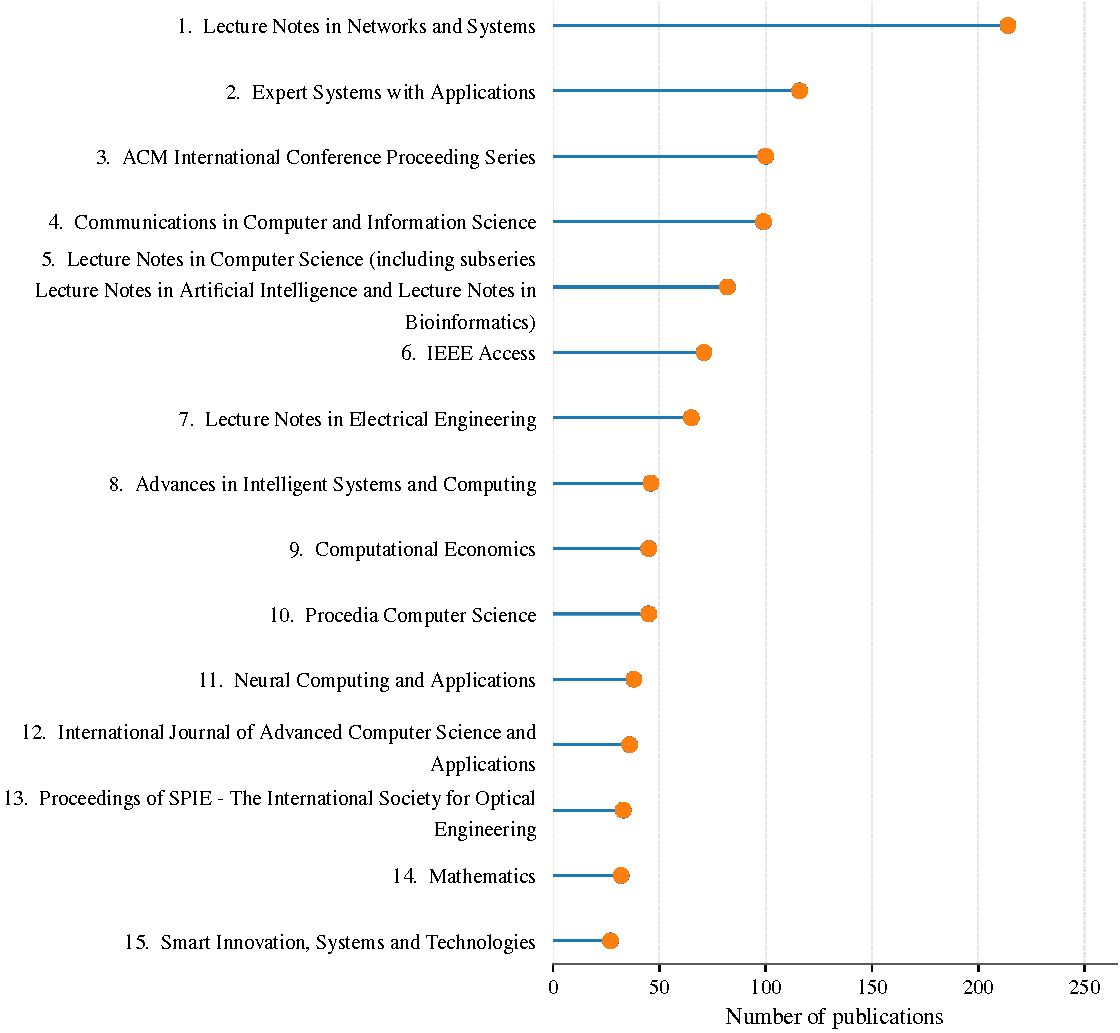
\includegraphics[
    width=0.96\linewidth
]{Fig3_Top15_Publication_Sources_Ranked_DotPlot_Q1.pdf}

\caption{Top publication sources in computational stock-market
forecasting based on the deduplicated bibliometric corpus.}
\label{fig:supp-top-sources}
\end{figure}

\FloatBarrier

% \subsection{Highly cited documents}
% \label{sec:supp-cited-documents}

\begin{table*}[!t]
\centering
\caption{Most highly cited documents among the Scopus-indexed records
retained in the deduplicated bibliometric corpus.}
\label{tab:supp-cited-documents}

\small
\setlength{\tabcolsep}{3.5pt}
\renewcommand{\arraystretch}{1.15}

\begin{tabular}{@{}rp{6.8cm}rp{4.5cm}r@{}}
\toprule
Rank &
Title &
Year &
Source &
Citations \\
\midrule

1 &
Financial time series forecasting using support vector machines &
2003 &
Neurocomputing &
1,439 \\

2 &
Stock price prediction using LSTM, RNN and CNN-sliding window model &
2017 &
International Conference on Advances in Computing,
Communications and Informatics (ICACCI 2017) &
959 \\

3 &
A hybrid ARIMA and support vector machines model in stock price
forecasting &
2005 &
Omega &
823 \\

4 &
Deep learning for event-driven stock prediction &
2015 &
IJCAI International Joint Conference on Artificial Intelligence &
747 \\

5 &
Deep learning networks for stock market analysis and prediction:
Methodology, data representations, and case studies &
2017 &
Expert Systems with Applications &
721 \\

6 &
Surveying stock market forecasting techniques--Part II:
Soft computing methods &
2009 &
Expert Systems with Applications &
707 \\

7 &
Textual analysis of stock market prediction using breaking
financial news: The AZFin text system &
2009 &
ACM Transactions on Information Systems &
678 \\

8 &
A comprehensive comparative study of artificial neural network
(ANN) and support vector machines (SVM) on stock forecasting &
2023 &
Annals of Data Science &
652 \\

9 &
Using artificial neural network models in stock market index
prediction &
2011 &
Expert Systems with Applications &
646 \\

10 &
A CNN-BiLSTM-AM method for stock price prediction &
2021 &
Neural Computing and Applications &
595 \\
\bottomrule
\end{tabular}

\vspace{2pt}
\begin{minipage}{0.97\textwidth}
\footnotesize
\textit{Note:} The ranking was calculated from the 4,789
Scopus-indexed records retained in the cross-database deduplicated
corpus. Citation counts were not combined across Scopus,
Web of Science, and IEEE Xplore. Publication years correspond to
the final source or proceedings year recorded in Scopus.
\end{minipage}
\end{table*}
\FloatBarrier

\paragraph{Interpretation of citations and family assignments.}
The citations included in Sections~S10.1--S10.10 illustrate
architectures, applications, and methodological issues and should
not be interpreted as complete one-to-one enumerations of
principal-family membership. The complete mapping of all coded
studies to study identifiers, citation keys, principal method
families, publication periods, and evidence scopes is provided in
Supplementary Data~S1.

% ============================================================
% S10. EXTENDED METHOD-FAMILY DISTRIBUTION
% ============================================================

\section{Extended method-family distribution}
\label{sec:supp-extended-technical}

This section provides the detailed period-wise distribution of the
principal computational-method families used in the
\(485\)-study technical-synthesis subset. The validation-design,
methodological-dimension, input-modality-recoverability, and
method-family-reliability tables are retained in the main manuscript
because they support the principal methodological conclusions of the
review.

\subsection{Method-family distribution across publication periods}
\label{sec:supp-family-period}

The period-wise distribution shows how the principal computational families
were represented across the four publication intervals used for the technical
synthesis. The period totals were 27 studies in 2016--2020, 36 in 2021--2022,
47 in 2023--2024, and 375 in 2025--2026, yielding the complete \(n=485\)
technical-synthesis subset.

\begin{table}[!htbp]
\centering\footnotesize
\caption{Frozen method-family distribution by technical-synthesis publication period ($n=485$).}
\label{tab:supp-family-period-new}
\setlength{\tabcolsep}{3.5pt}
\begin{tabularx}{\linewidth}{@{}>{\RaggedRight\arraybackslash}Xrrrrr@{}}
\toprule
Principal family & 2016--20 & 2021--22 & 2023--24 & 2025--26 & Total \\
\midrule
Deep-learning models & 11 & 10 & 23 & 70 & 114 \\
Hybrid deep-learning models & 4 & 10 & 6 & 89 & 109 \\
Sentiment/NLP-driven models & 4 & 8 & 5 & 60 & 77 \\
Transformer/attention-based models & 0 & 1 & 7 & 60 & 68 \\
Metaheuristic-optimized models & 7 & 3 & 2 & 39 & 51 \\
Ensemble/tree-based machine learning & 1 & 3 & 2 & 26 & 32 \\
Graph-based models & 0 & 0 & 2 & 14 & 16 \\
Multimodal-fusion models & 0 & 0 & 0 & 12 & 12 \\
Other/unclear & 0 & 1 & 0 & 2 & 3 \\
ANN/neuro-fuzzy models & 0 & 0 & 0 & 2 & 2 \\
Statistical/econometric models & 0 & 0 & 0 & 1 & 1 \\
\midrule
Total & 27 & 36 & 47 & 375 & 485 \\
\bottomrule\end{tabularx}
\end{table}
\FloatBarrier

\subsection{Deep-learning models}
\label{sec:supp-deep-learning}

Deep-learning models \cite{P00021,P00042,P00044,P00056,P00063,P00077,P00078,P00114,P00162,P00191,P00202,P00233,P03420,P03475,P03576,P03634,P03654,P03661,P03870,P03943,P04100,P04285} constituted the largest principal family
($n=114$, 23.5\%) in the frozen technical-synthesis subset. The family
included recurrent \cite{P00235,P00251,P00277,P00317,P00348,P00353,P00370,P00416,P00439,P00452,P00464,P00471}, long short-term memory networks \cite{P00489,P00564,P00570,P00576,P00587,P00645,P00646,P00649,P00650,P00652,P00656,P00661}, gated recurrent units \cite{P00671,P00677,P00730,P00739,P00750,P00765,P00791,P00811,P00821,P00826,P00829,P00834}, convolutional \cite{P00851,P00852,P00935,P00940,P00976,P01023,P01056,P01062,P01116,P01123,P01155}, temporal \cite{P01182,P01195,P01229,P01231,P01233,P01323,P01371,P01437,P01471,P01487,P01495,P01551}, autoencoding \cite{P01589,P01637,P01849,P01885,P01901,P01911,P01953,P02051,P02056,P02095,P02138,P02139}, and related
representation-learning architectures \cite{P02220,P02244,P02639,P02878,P02922,P02943,P02950,P03089,P03221,P03226,P03384,P03397}. Their principal methodological
advantages lie in nonlinear sequential representation learning, while the
reviewed evidence emphasizes continuing concerns regarding temporal
validation, preprocessing boundaries, baseline strength, statistical
comparison, and reproducibility.

\subsection{Hybrid deep-learning models}
\label{sec:supp-hybrid-deep-learning}

Hybrid deep-learning models formed the second-largest principal family,
comprising 109 studies (22.5\%) of the technical-synthesis subset.
This family included forecasting pipelines that explicitly integrated two
or more modelling, representation, decomposition, optimization, or
information-fusion components. Common configurations combined convolutional \cite{P00930,P00931,P00943}
or recurrent sequence modelling with attention \cite{P00015,P00020,P00022,P00030,P00037,P00072,P00092,P00099,P00117,P00124,P00130,P00140}, decomposition \cite{P00321,P00334,P00339,P00346,P00366,P00373,P00390,P00394,P00410,P00413,P00415,P00419,P01245,P01290,P01429,P01591,P01708,P01936,P02257,P02398,P02416,P02517,P02669,P02696}, textual
information \cite{P00421,P00425,P00434,P00435,P00443,P00444,P00447,P00450,P00466,P00467,P00488,P00501}, or optimization-assisted components \cite{P00506,P00510,P00519,P00537,P00543,P00553,P00554,P00560,P00569,P00572,P00584,P00633}.


The principal methodological challenge of hybridization is attribution.
Representative configurations include CNN--LSTM~\cite{P00673,P00685,P00705,P00745,P00752,P00763,P00775,P00807,P00838,P00842,P00845,P00846},
CNN--GRU~\cite{P00860,P00866,P00872,P00878,P00890,P00891,P00909,P00910,P00930,P00931,P00943,P00947}, bidirectional recurrent architectures~\cite{P00951,P00956,P00964,P00974,P00984,P01069,P01082,P01094,P01112,P01126,P01131,P01168},
decomposition followed by deep sequence modelling~\cite{P02877,P02956,P02991,P02999,P03006,P03106,P03317,P03366,P03386,P03508,P03964,P04069},
attention-enhanced recurrent networks~\cite{P00220,P00228,P00237,P00250}, and deep models optimized
through metaheuristics~\cite{P03366,P03386,P03508}. When several components are introduced
simultaneously, performance gains cannot be assigned reliably to an individual
component without controlled ablation.


Fair evaluation therefore requires component-wise ablations under
identical training, validation, and test periods, together with comparable
tuning budgets. Data-dependent decomposition, feature selection, and
normalization should also be restricted to training information. The
concentration of hybrid approaches in the recent prioritized evidence base
indicates rapid methodological uptake, but does not by itself establish
superior generalization, economic utility, or robustness.

\subsection{Sentiment and NLP-driven models}
\label{sec:supp-sentiment-nlp}

Sentiment- and NLP-driven models accounted for 77 studies (15.9\%) and
treated textual interpretation \cite{P00070,P00088,P00098,P00108,P00141}, sentiment construction \cite{P03037,P03139,P03350,P03353,P03705,P03742,P03834,P03861,P03966,P04573}, event extraction \cite{P01662,P02324,P02642,P02841},
language representation \cite{P00832,P00854,P00907}, or text--market integration \cite{P00011,P00046,P00059,P00070,P00088,P00098,P00108,P00141,P00146,P00157,P00178,P00201} as the principal
methodological contribution. The family included conventional sentiment
representations \cite{P00213,P00224,P00253,P00254,P00261,P00267,P00296,P00307,P00343,P00367,P00380} as well as neural \cite{P00797,P00832,P00854,P00907,P00944,P00965,P00970,P01048,P01060,P01120,P01125,P01169,P01198,P01224,P01228,P01276,P01304,P01500,P01662,P02324,P02642,P02841,P02918,P02948} and transformer-based textual encoders \cite{P00388,P00411,P00495,P00544,P00561,P00577,P00585,P00597,P00601,P00603,P00605,P00611,P00625,P00639,P00647,P00706,P00708,P00722,P00725,P00726,P00758,P00778}.

These 77 principal-family assignments should not be interpreted as equivalent
to the input-modality counts reported in the main manuscript. Textual and
social-media modalities were coded non-mutually exclusively and could also
occur in studies principally classified as hybrid, transformer, graph,
ensemble, or multimodal approaches.

The central methodological requirement for text-based forecasting is
point-in-time alignment. Publication timestamps, market-session alignment,
time zones, document deduplication, entity matching, aggregation rules, and
text-source provenance should be reported sufficiently to establish that no
document or sentiment label incorporates information unavailable at the
forecasting origin. Market-only and leave-text-out baselines are particularly
useful for establishing the incremental contribution of textual information.

\subsection{Transformer and attention-based models}
\label{sec:supp-transformers}

Transformer- and attention-based models accounted for 68 studies (14.0\%).
Their representation in the prioritized technical subset increased sharply,
from 1 study in 2021--2022 and 7 in 2023--2024 to 60 in 2025--2026.
This concentration indicates rapid recent uptake, although it should not be
interpreted as a complete historical enumeration of attention-based financial
forecasting.

These approaches were used to model temporal dependencies \cite{P00040,P00062,P00089,P00107} and interactions
among historical observations \cite{P00189,P00282,P00291}, technical variables \cite{P00303,P00331,P00364,P00377,P00385}, textual signals \cite{P00403,P00451,P00517,P00571,P00579}, assets \cite{P00635,P00687,P00707,P00831,P00858,P00876,P00895},
graph neighbours \cite{P00896,P00938,P00966}, and multimodal representations \cite{P01035,P01084,P01137,P01187,P01193,P01424,P01738,P02987,P04538}. Their methodological
validity nevertheless depends on the same information constraints as other
forecasting architectures. Causal masking, target alignment, normalization,
sequence construction, and hyperparameter selection should prevent future
information from entering the forecasting representation. Comparisons should
also control for model complexity and tuning effort. Where attention weights
are interpreted as explanatory evidence, their stability across periods and
model configurations should be examined rather than treating attention
weights as causal explanations.

\subsection{Metaheuristic-optimized models}
\label{sec:supp-metaheuristics}

Metaheuristic-optimized models accounted for 51 studies (10.5\%). These
approaches used evolutionary \cite{P00923,P00962,P01021,P01055,P01089,P01214}, swarm-based \cite{P01687,P01785,P02381,P02464,P02563,P02976}, physics-inspired \cite{P03101,P03518,P03885,P03886,P03936,P04110,P04194}, or related
population-based search procedures for feature selection, hyperparameter
optimization, architecture search, weight or decomposition-parameter tuning,
threshold selection, or multi-objective model design.

Their principal methodological risk is validation overfitting. Repeated
evaluation of candidate configurations against the same validation or test
period can adapt the search process to that period even when the optimizer
is gradient-free. Reliable evaluation should therefore separate optimization
from final testing through temporally ordered training--validation procedures
and an untouched outer test period. Search population \cite{P00035,P00049,P00061,P00129,P00163}, iterations \cite{P00196,P00216,P00259,P00274,P00285,P00312,P00345}, stopping
criteria \cite{P00355,P00362,P00369,P00392}, random seeds \cite{P00536,P00540,P00562,P00563}, objective functions \cite{P00592,P00595,P00610,P00614}, parameter bounds \cite{P00617,P00638,P00655,P00660,P00701}, and overall
evaluation budget \cite{P00774,P00810,P00830,P00857,P00865,P00886,P00920} should be reported. Comparisons should also control for
search effort and, where appropriate, include simpler tuning baselines.
Multi-objective studies should report the relevant trade-offs rather than
selecting a favourable solution after examination of test performance.

\subsection{Ensemble and tree-based machine learning}
\label{sec:supp-ensemble}

Ensemble \cite{P00401,P00509,P00551,P00600,P00608,P00651,P00654,P00688,P00690,P00698,P00734,P00744,P01034,P01167,P01208,P01249,P01269,P01324} and tree-based \cite{P00019,P00057,P00071,P00080,P00083,P00120,P00121,P00154,P00183,P00190,P00260,P00400,P00898,P00911,P00955,P00983,P00988,P01008} machine-learning approaches accounted for 32 studies
(6.6\%). The family included random forests, gradient-boosting methods,
boosted decision trees, bagging, voting, stacking, and related ensemble
configurations in which tree-based or ensemble learning formed the principal
methodological contribution.

These approaches are particularly suited to structured predictors such as
lagged market variables, technical indicators, macroeconomic information,
and accounting variables. Their validity nevertheless depends on temporal
construction of the complete learning pipeline. In stacking, second-level
models should be trained from out-of-sample predictions generated without
access to the corresponding future targets; randomly constructed folds may
otherwise introduce temporal leakage. Feature-importance \cite{P00749,P00751,P00759,P00767,P00769,P00773,P00796,P00824,P00825,P00833,P00853,P00863,P01582,P01663,P01837,P01978,P02751,P03242,P03277,P03347,P03446,P03540,P03726,P03799} results should also
be interpreted cautiously because correlated predictors and importance
definitions can substantially affect rankings. Temporal stability and
group-level interpretation are therefore more informative than a single
importance ranking obtained from one fitted sample.

\subsection{Graph-based models}
\label{sec:supp-graph}

Graph-based models accounted for 16 studies (3.3\%), including two studies
during 2023--2024 and 14 during 2025--2026. These approaches represented
securities, sectors, markets, events, or information sources as nodes linked
through economic, statistical, textual, or learned relationships.

The principal methodological issue is point-in-time graph construction.
Adjacency structures estimated using the complete dataset may incorporate
future correlations or relationships that were unavailable during training,
while retrospective use of current market constituents can introduce
survivorship bias. Graph-based studies \cite{P00050,P00151,P00186,P00248,P00293,P00297,P00414,P00513,P00674,P00727,P00753,P00816,P00879,P01043,P01281,P01732} should therefore document the economic
meaning of nodes and edges, construction window, update rule, directionality,
edge weighting, temporal availability, and treatment of changing
constituents. Where feasible, static, rolling, and learned graph structures
should be compared, and generalization should be evaluated across time,
assets, sectors, or markets rather than only through randomly separated
node--time observations.


\subsection{Multimodal-fusion models}
\label{sec:supp-multimodal}

Multimodal-fusion models \cite{P00144,P00160,P00420,P00552,P00642,P00663,P01052,P01135,P01260,P01263} accounted for 12 studies (2.5\%), all published
during 2025--2026 in the prioritized technical subset. These studies
explicitly integrated information from different modalities, including
market histories, technical indicators, textual sources, social media,
fundamentals, macroeconomic variables, and relational information.

The principal methodological challenge is temporal alignment across
heterogeneous information sources. Different modalities have different
publication times, update frequencies, missingness patterns, revision
policies, and source-validity constraints; consequently, every input should
be aligned with the information demonstrably available at the corresponding
forecasting origin. Multimodal evaluations should include market-only and
single-modality baselines, leave-one-modality-out ablations, and robustness
tests for missing or delayed information. Because all 12 principal
multimodal assignments occurred in the latest publication period, the
observed concentration should be interpreted as an emerging pattern in the
recent prioritized evidence base rather than evidence of field-wide
dominance.


\subsection{ANN, neuro-fuzzy, and other approaches}
\label{sec:supp-other-models}

Two studies (0.4\%) \cite{P00841,P01112} were classified principally as a conventional artificial
neural-network or neuro-fuzzy contribution, and three studies (0.6\%)
remained in the Other or unclear category. These small counts do not imply that
artificial neural networks, fuzzy systems, or unconventional models
were historically unimportant.

The bibliometric and thematic analyses showed that artificial neural
networks and computational intelligence formed major intellectual
foundations of the field. Their small representation in the technical
taxonomy results from two features of the coding design. First, each
study received only one principal-family assignment. Second, the
technical subset is dominated by recent publications whose principal
contributions were more frequently framed as deep, hybrid,
transformer, sentiment, graph, optimization, or multimodal models.

Conventional neural or fuzzy components may therefore appear inside
other families without being counted separately. The other or unclear
category was retained only when the available evidence did not support
a more defensible principal-family assignment.

These sparse categories should remain visible rather than being merged
post hoc into larger groups, because doing so would conceal genuine
coding uncertainty and weaken the auditability of the taxonomy.

\subsection{Statistical and econometric models}
One study (0.2\%) was classified principally as a statistical/econometric
method, reflecting the implemented ARIMA-only forecasting experiment \cite{P00211}.
This residual category is maintained independently instead of being
absorbed into a deep-learning or hybrid category. This small proportion
reflects the recent purposively prioritized technical sample and should
not be read as the field-wide historical prevalence of statistical
forecasting approaches.

\subsection{Cross-family methodological reliability}

Across the principal computational-method families, architectural
sophistication was not consistently accompanied by stronger methodological
evidence. Temporally ordered validation, training-only preprocessing,
economic evaluation, formal statistical testing, and public code availability
remained limited across several families. Table~\ref{tab:family-reliability}
provides the complete family-level reliability profile derived from the frozen
\(n=485\) technical-synthesis register.

% Table~\ref{tab:family-period} reports the complete family-by-period
% distribution.

\begin{landscape}
\begin{table}[!p]
\centering
\caption{Principal method-family profile of evidence-supported reliability practices in the frozen $n=485$ technical-synthesis subset.}
\label{tab:family-reliability}
\scriptsize
\setlength{\tabcolsep}{2.4pt}
\renewcommand{\arraystretch}{1.12}
\begin{tabularx}{\linewidth}{@{}>{\RaggedRight\arraybackslash}p{3.5cm}r*{6}{>{\centering\arraybackslash}X}@{}}
\toprule
Method family & Studies & Temporal validation & Training-only prep. & High leakage risk & Economic eval. & Formal tests & Code available \\
\midrule
Deep-learning models & 114 & 12 (10.5\%) & 3 (2.6\%) & 6 (5.3\%) & 6 (5.3\%) & 7 (6.1\%) & 1 (0.9\%) \\
Hybrid deep-learning models & 109 & 14 (12.8\%) & 3 (2.8\%) & 9 (8.3\%) & 8 (7.3\%) & 12 (11.0\%) & 2 (1.8\%) \\
Sentiment/NLP-driven models & 77 & 15 (19.5\%) & 6 (7.8\%) & 5 (6.5\%) & 7 (9.1\%) & 7 (9.1\%) & 0 (0.0\%) \\
Transformer/attention-based models & 68 & 18 (26.5\%) & 5 (7.4\%) & 5 (7.4\%) & 8 (11.8\%) & 7 (10.3\%) & 3 (4.4\%) \\
Metaheuristic-optimized models & 51 & 8 (15.7\%) & 2 (3.9\%) & 2 (3.9\%) & 2 (3.9\%) & 5 (9.8\%) & 0 (0.0\%) \\
Ensemble/tree-based machine learning & 32 & 8 (25.0\%) & 0 (0.0\%) & 3 (9.4\%) & 2 (6.2\%) & 5 (15.6\%) & 1 (3.1\%) \\
Graph-based models & 16 & 4 (25.0\%) & 2 (12.5\%) & 1 (6.2\%) & 2 (12.5\%) & 3 (18.8\%) & 0 (0.0\%) \\
Multimodal-fusion models & 12 & 0 (0.0\%) & 0 (0.0\%) & 1 (8.3\%) & 2 (16.7\%) & 1 (8.3\%) & 0 (0.0\%) \\
Other/unclear & 3 & 1 (33.3\%) & 0 (0.0\%) & 0 (0.0\%) & 0 (0.0\%) & 1 (33.3\%) & 0 (0.0\%) \\
ANN/neuro-fuzzy models & 2 & 1 (50.0\%) & 0 (0.0\%) & 0 (0.0\%) & 0 (0.0\%) & 0 (0.0\%) & 0 (0.0\%) \\
Statistical/econometric models & 1 & 0 (0.0\%) & 0 (0.0\%) & 0 (0.0\%) & 0 (0.0\%) & 0 (0.0\%) & 0 (0.0\%) \\
\textbf{Total} & \textbf{485} & 81 (16.7\%) & 21 (4.3\%) & 32 (6.6\%) & 37 (7.6\%) & 48 (9.9\%) & 7 (1.4\%) \\
\bottomrule
\end{tabularx}
\vspace{1mm}
\begin{minipage}{\linewidth}\footnotesize
\textit{Note.} Within-family percentages use the row denominator;
percentages in the total row use $n=485$. ``Unclear'' is not confirmation of absence.
\end{minipage}
\end{table}

\end{landscape}

\FloatBarrier



\section{Extended limitations and sensitivity analyses}
\label{sec:supp-limitations-and-sensitivity-analyses}

This section reports the complete review-level limitations, interpretive
boundaries, and sensitivity considerations supporting the concise limitations statement retained in the main article.

\subsection{Review limitations and interpretive boundaries}

The complete review-level limitations, their possible influences, the
mitigation measures adopted in the review, and the corresponding interpretive
boundaries are summarized in Table~\ref{tab:review-limitations}.

% \input{tables/Table19_review_limitations}

\begin{landscape}

\small
\setlength{\tabcolsep}{4pt}
\renewcommand{\arraystretch}{1.15}

\begin{longtable}{
@{}
L{0.19\linewidth}
L{0.245\linewidth}
L{0.245\linewidth}
L{0.245\linewidth}
@{}
}

\caption{Review limitations, possible influences, existing
mitigations, and interpretive boundaries.}
\label{tab:review-limitations}
\\

\toprule
\textbf{Review limitation} &
\textbf{Possible influence} &
\textbf{Existing mitigation} &
\textbf{Interpretive boundary}
\\
\midrule
\endfirsthead

\multicolumn{4}{c}{%
\tablename\ \thetable\ continued from the previous page}
\\
\toprule
\textbf{Review limitation} &
\textbf{Possible influence} &
\textbf{Existing mitigation} &
\textbf{Interpretive boundary}
\\
\midrule
\endhead

\midrule
\multicolumn{4}{r}{Continued on the next page}
\\
\endfoot

\bottomrule
\endlastfoot

Purposefully prioritized \(485\)-study technical-synthesis subset
&
The technical distributions may overrepresent recent studies and
records for which methodological information was comparatively
recoverable.
&
The prioritization, eligibility, evidence-recovery, and
representativeness procedures are reported explicitly.
&
The technical-synthesis distributions should not be interpreted as
probability-based estimates of field-wide prevalence.
\\
\addlinespace[3pt]

Strong concentration of recent studies
&
A total of \(375\) of the \(485\) studies (\(77.3\%\)) were published
during 2025--2026. Recent architectures and reporting practices
therefore dominate the technical synthesis.
&
Long-term intellectual and methodological development was analysed
separately using the broader four-decade bibliometric corpus.
&
Recent technical evidence should be distinguished from historical
field-wide trends when interpreting methodological evolution.
\\
\addlinespace[3pt]

Mixed evidence scope
&
The \(85\) abstract-only and \(25\) metadata-only records provide less
methodological detail than the \(375\) full-text records.
&
Evidence scope was recorded for every study, and claims were restricted
to information recoverable from the corresponding evidence source.
&
An \textit{Unclear} classification denotes insufficient evidence and
should not be interpreted as confirmation that a practice was absent.
\\
\addlinespace[3pt]

Database- and index-specific coverage
&
Venue, disciplinary, regional, and document-type coverage may differ
across bibliographic databases and indexing systems.
&
Multiple scholarly databases, explicit search protocols, and systematic
cross-database deduplication were used to broaden coverage.
&
The findings characterize the indexed and screened corpus rather than
all published, unpublished, or grey literature.
\\
\addlinespace[3pt]

Partial coverage of 2026
&
The 2026 publication total represents an incomplete year and may create
the appearance of declining annual research output.
&
The partial-year status was identified explicitly, and 2026 records
were excluded from complete-year thematic-evolution analysis where
appropriate.
&
The 2026 publication count should not be interpreted as evidence of
declining research activity.
\\
\addlinespace[3pt]

Citation-age bias
&
Older studies have had more time to accumulate citations than recent
publications, particularly those published during 2025--2026.
&
Citation patterns were interpreted alongside publication year and
complemented by thematic, network, and methodological evidence.
&
Citation frequency should not be equated directly with current
methodological quality, reliability, or practical relevance.
\\
\addlinespace[3pt]

Absence of formal inter-reviewer Cohen's \(\kappa\)
&
The consistency of screening and coding decisions cannot be summarized
using a chance-corrected inter-reviewer agreement coefficient.
&
A stratified \(40\)-study verification exercise was conducted, and
ambiguous classifications were resolved through manual adjudication.
&
The \(37/40\) confirmation result (\(92.5\%\)) is a raw confirmation
rate and must not be reported as Cohen's \(\kappa\).
\\  

\bottomrule
\end{longtable}
\end{landscape}

\FloatBarrier

\subsection{Sensitivity and interpretive scope}

Evidence recoverability differed across full-text, abstract-only, and
metadata-only records; accordingly, an \textit{Unclear} classification
indicates insufficient recoverable evidence rather than confirmed absence
of a methodological practice. Because the 485-study technical subset was
purposively prioritized and strongly concentrated in recent publications,
its study-level distributions describe the selected technical evidence base
and should not be interpreted as probability-based field-wide prevalence
estimates.
% ============================================================
% CONSOLIDATED SUPPLEMENTARY REFERENCES
% ============================================================

\FloatBarrier
\clearpage

\bibliographystyle{sn-basic}
\bibliography{sn-bibliography}

\end{document}